\section{Results}
\label{sec:results}

\begin{figure}[t]
    \centering
    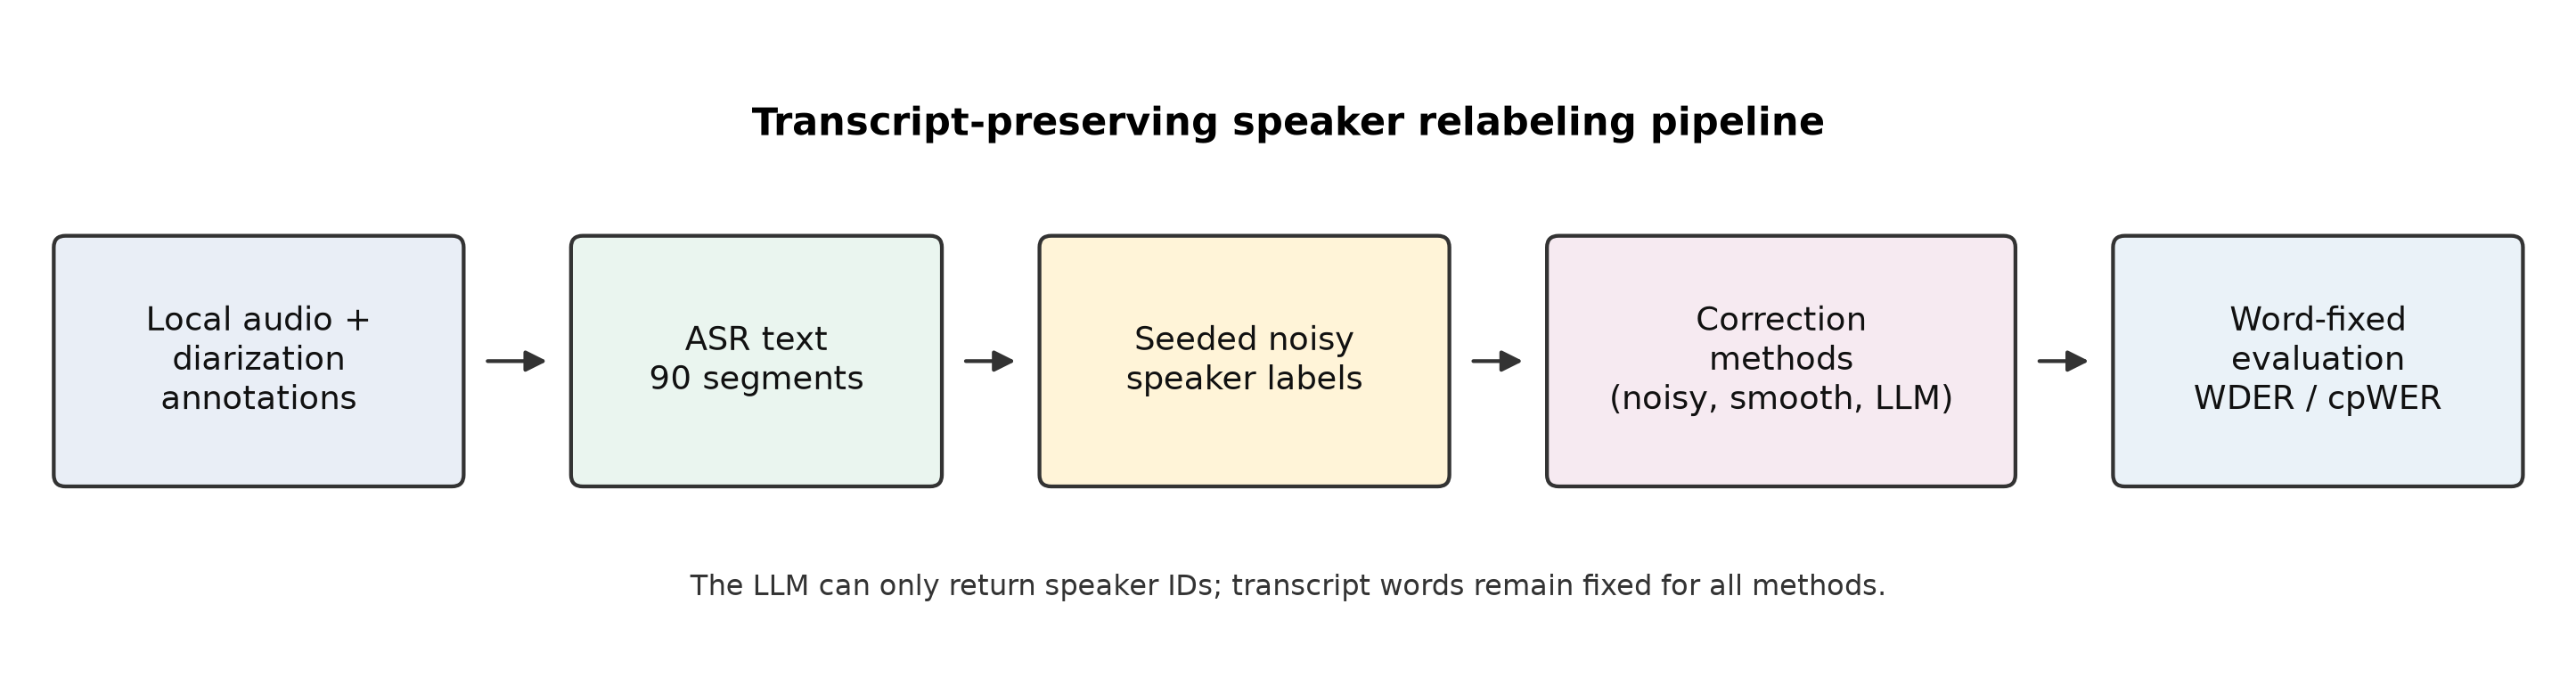
\includegraphics[width=0.95\linewidth]{figures/method_overview.png}
    \caption{Overview of the transcript-preserving pilot. We transcribe real audio segments, inject seeded speaker-label noise, run deterministic and LLM correction methods, and evaluate speaker labels while keeping transcript words fixed.}
    \label{fig:method}
\end{figure}

\para{Overall performance.} \Tabref{tab:main_results} shows the aggregate results across 30 window/noise cases. \llmnoprofile achieves the lowest mean \wder (0.375) and mean \cpwer (0.521), improving over \noisylabels by 0.015 WDER and 0.030 cpWER. \llmprofile is slightly weaker, with mean \wder 0.381 and mean \cpwer 0.529. \smooth performs worst on WDER and segment error, showing that simple local continuity is not a reliable substitute for speaker-aware reasoning.

\begin{table}[t]
    \centering
    \resizebox{\textwidth}{!}{%
    \begin{tabular}{@{}lrrrrr@{}}
        \toprule
        \textbf{Method} & \textbf{Mean WDER} $\downarrow$ & \textbf{Mean cpWER} $\downarrow$ & \textbf{Segment err.} $\downarrow$ & \textbf{Speaker-count MAE} $\downarrow$ & \textbf{Parse success} \\
        \midrule
        \llmnoprofile       & {\bf 0.375} & {\bf 0.521} & {\bf 0.373} & {\bf 0.400} & 1.00 \\
        \llmprofile         & 0.381       & 0.529       & 0.380       & {\bf 0.400} & 1.00 \\
        \noisylabels        & 0.390       & 0.550       & 0.387       & {\bf 0.400} & 1.00 \\
        \smooth             & 0.442       & 0.628       & 0.437       & {\bf 0.400} & 1.00 \\
        \bottomrule
    \end{tabular}
    }
    \caption{Overall results across 30 window/noise cases. Lower is better for WDER, cpWER, segment error, and speaker-count MAE. Best values are in \textbf{bold}. \llmnoprofile gives the best mean accuracy, but the margin over \noisylabels is small.}
    \label{tab:main_results}
\end{table}


\para{Dataset split.} The overall mean hides a clear split by speaker count and dataset. In \amisdm, both LLM conditions exactly match \noisylabels on mean \wder (0.443) and mean \cpwer (0.630). In \simsamu, \llmnoprofile reduces mean \wder from 0.310 to 0.273 and mean \cpwer from 0.431 to 0.357. This supports the narrower claim that prompted LLMs can correct some two-speaker transcript-context errors, but weakens the broader hypothesis for four-speaker meeting identification.

\begin{table}[t]
    \centering
    \resizebox{\textwidth}{!}{%
    \begin{tabular}{@{}llrrr@{}}
        \toprule
        \textbf{Dataset} & \textbf{Method} & \textbf{Speakers} & \textbf{Mean WDER} $\downarrow$ & \textbf{Mean cpWER} $\downarrow$ \\
        \midrule
        \amisdm & \noisylabels  & 4 & {\bf 0.443} & 0.630 \\
        \amisdm & \llmnoprofile & 4 & {\bf 0.443} & 0.630 \\
        \amisdm & \llmprofile   & 4 & {\bf 0.443} & 0.630 \\
        \amisdm & \smooth       & 4 & 0.453       & {\bf 0.626} \\
        \midrule
        \simsamu & \noisylabels  & 2 & 0.310       & 0.431 \\
        \simsamu & \llmnoprofile & 2 & {\bf 0.273} & {\bf 0.357} \\
        \simsamu & \llmprofile   & 2 & 0.287       & 0.379 \\
        \simsamu & \smooth       & 2 & 0.425       & 0.631 \\
        \bottomrule
    \end{tabular}
    }
    \caption{Dataset split. The LLM gain is concentrated in the two-speaker \simsamu condition. In four-speaker \amisdm, both LLM conditions leave aggregate WDER and cpWER unchanged relative to \noisylabels.}
    \label{tab:dataset_split}
\end{table}


\para{Statistical evidence.} \Tabref{tab:stats} reports paired tests against \noisylabels. No correction method achieves a statistically significant WDER improvement after Holm correction. \llmnoprofile has a positive mean WDER reduction of 0.015, but its 95\% bootstrap interval includes zero ($[-0.009, 0.045]$), and the Holm-adjusted $p$-value is 0.410. \llmprofile shows an even smaller mean reduction of 0.009. \smooth has a negative reduction, meaning it increases mean WDER relative to \noisylabels.

\begin{table}[t]
    \centering
    \resizebox{\textwidth}{!}{%
    \begin{tabular}{@{}lrrrrr@{}}
        \toprule
        \textbf{Comparison} & \textbf{Mean WDER red.} & \textbf{95\% CI} & \textbf{Test} & \textbf{$p$} & \textbf{Holm $p$} \\
        \midrule
        \noisylabels vs. \smooth       & -0.052 & $[-0.101, -0.008]$ & Wilcoxon & 0.978 & 0.978 \\
        \noisylabels vs. \llmnoprofile & {\bf 0.015} & $[-0.009, 0.045]$ & Wilcoxon & 0.137 & 0.410 \\
        \noisylabels vs. \llmprofile   & 0.009 & $[-0.001, 0.029]$ & Wilcoxon & 0.327 & 0.655 \\
        \bottomrule
    \end{tabular}
    }
    \caption{Paired WDER tests over 30 case pairs. Positive reduction means the method improves over \noisylabels. No correction method reaches statistical significance after Holm correction.}
    \label{tab:stats}
\end{table}


\para{Conservatism and parse reliability.} The LLM did not fail structurally: all 60 responses parsed successfully. The main failure mode is conservatism. \llmnoprofile leaves 26/30 cases unchanged, improves 3, and worsens 1. \llmprofile leaves 28/30 cases unchanged, improves 1, and worsens 1. \Figref{fig:wder_by_method} and \figref{fig:dataset_reduction} show the same pattern visually: the average LLM gain is small, concentrated in \simsamu, and absent in \amisdm.

\begin{figure}[t]
    \centering
    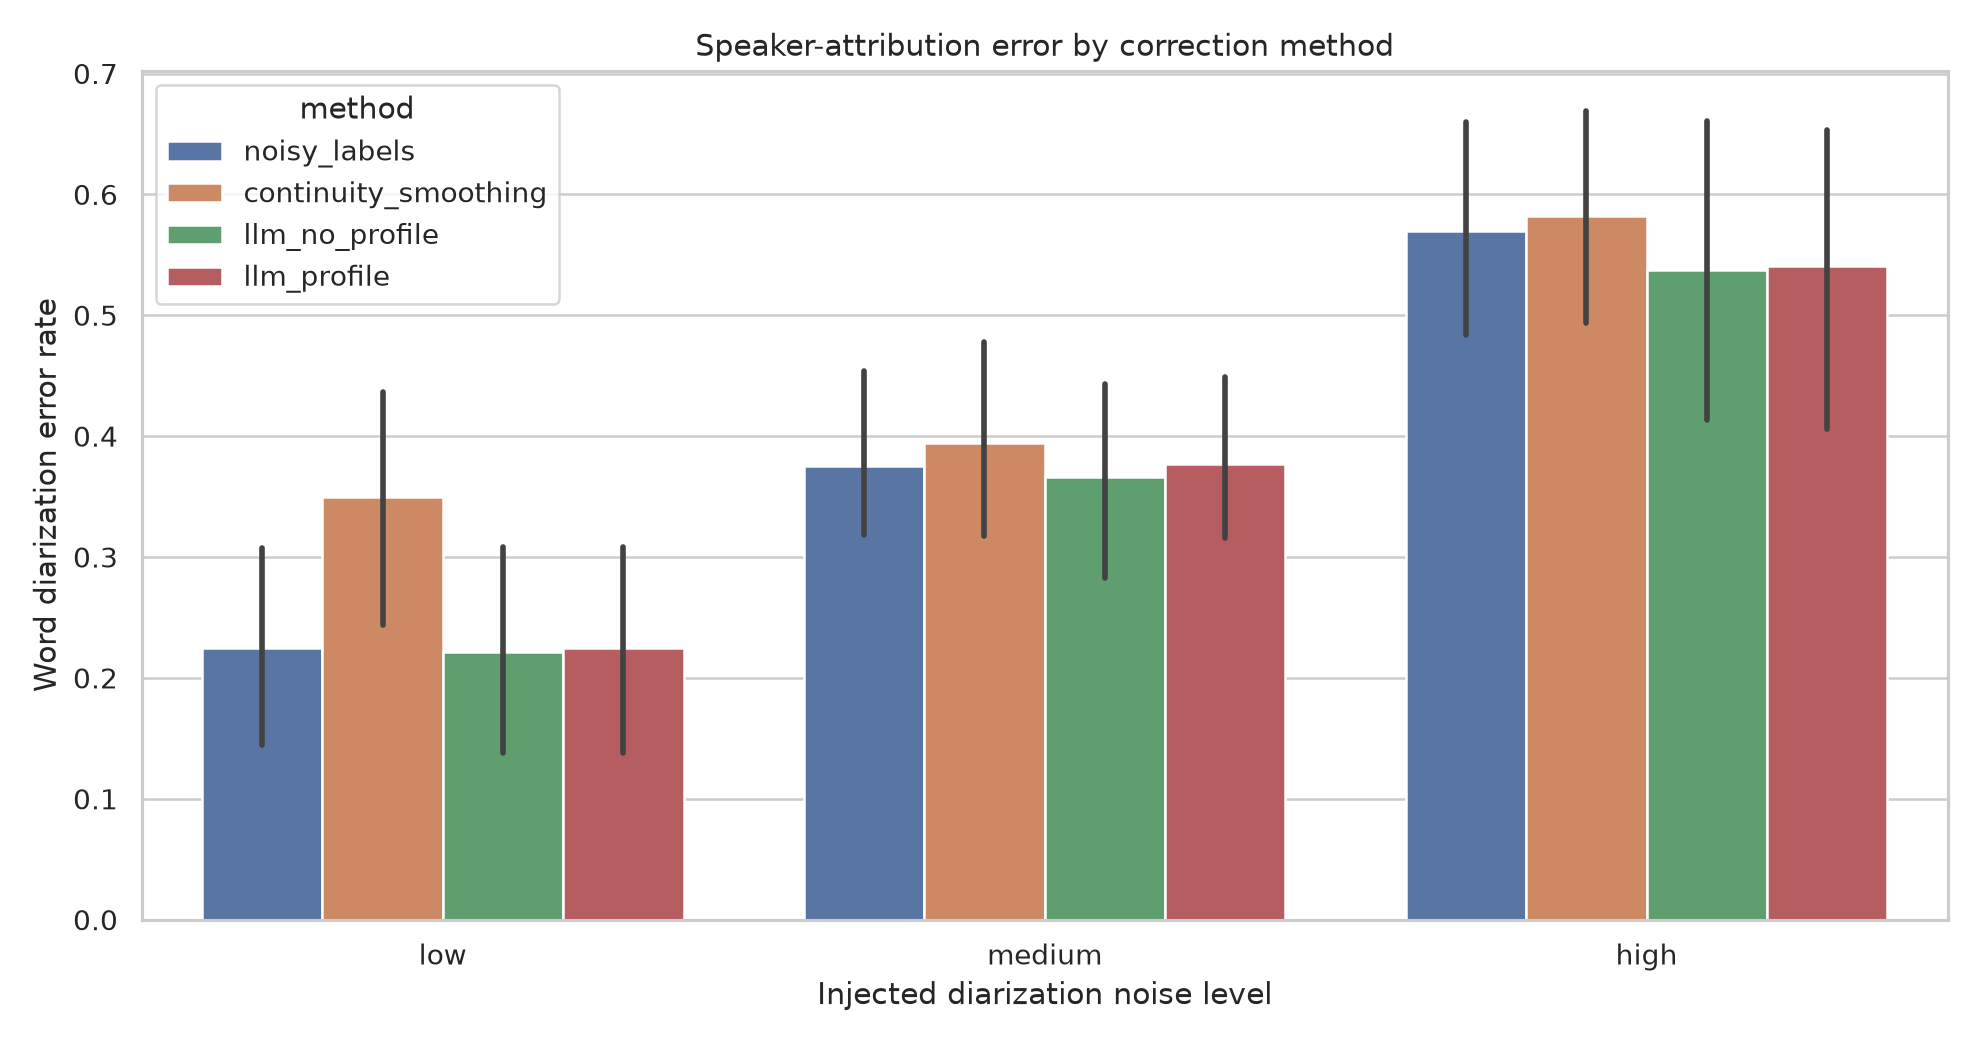
\includegraphics[width=0.95\linewidth]{figures/wder_by_method.png}
    \caption{WDER by method across all 30 cases. Lower is better. \llmnoprofile has the best mean WDER, but the improvement over \noisylabels is small and not statistically significant.}
    \label{fig:wder_by_method}
\end{figure}

\begin{figure}[t]
    \centering
    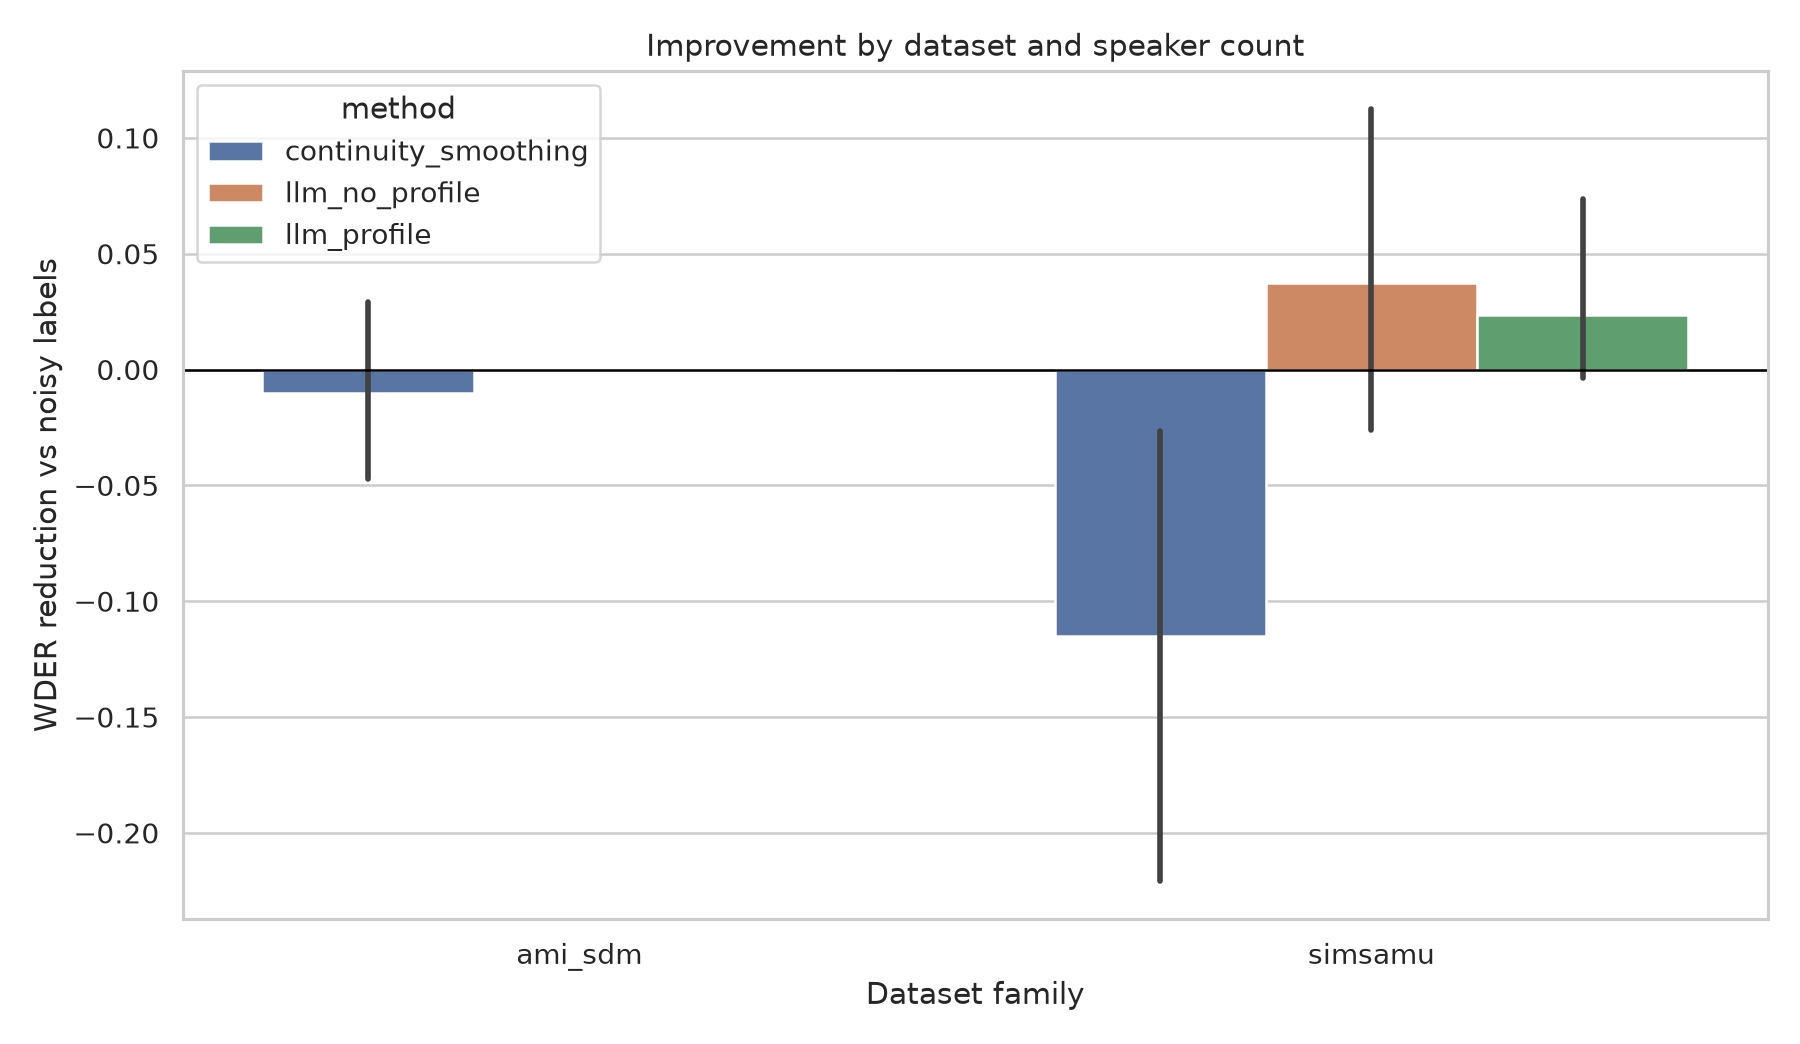
\includegraphics[width=0.95\linewidth]{figures/wder_reduction_by_dataset.png}
    \caption{WDER reduction relative to \noisylabels by dataset. Positive values mean improvement. LLM gains appear in the two-speaker \simsamu setting, while the four-speaker \amisdm setting shows no LLM reduction.}
    \label{fig:dataset_reduction}
\end{figure}

\begin{figure}[t]
    \centering
    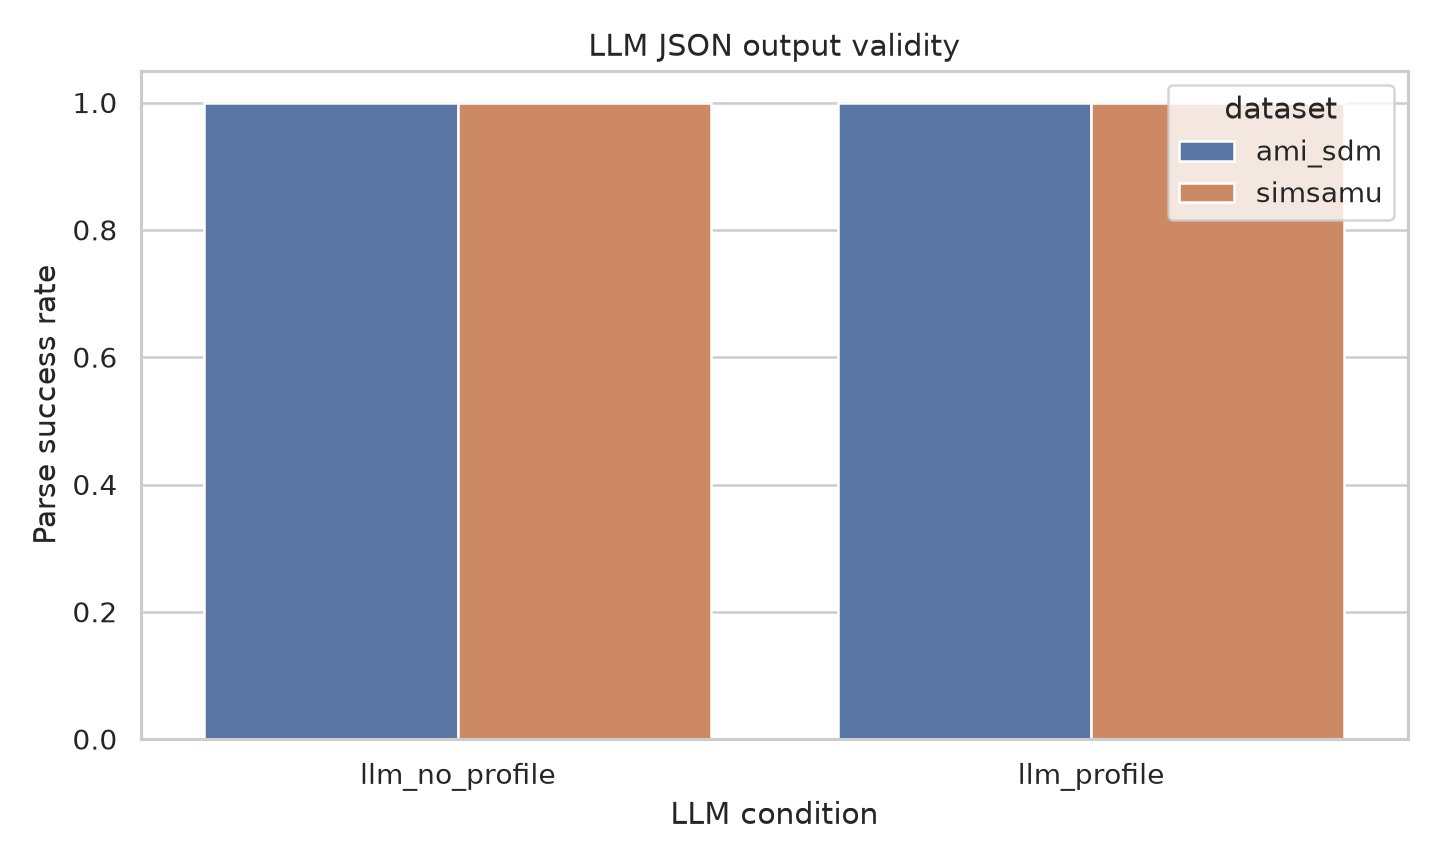
\includegraphics[width=0.8\linewidth]{figures/llm_parse_success.png}
    \caption{LLM parse success. Both LLM conditions return valid JSON assignments for every call, so the limiting factor is not output formatting but whether the model changes incorrect labels.}
    \label{fig:parse_success}
\end{figure}
